%%%%%%%%%%%%%%%%%%%%%%%%%%%%%
%Algorithmen zur Lösung???

%Schreibweise: Kernel oder Kerne??

%SKALARES PROBLEM?

%Verweis auf voriges Kapitel + Klärung der Begriffe n_f, N_eff nicht vergessen!

%Ausblick   + Algorithmus (evtl extra Kapitel mit sachen zur implementierung und bildern)

%diagramme nicht vergessen
%%%%%%%%%%%%%%%%%%%%%%%%%%%%%
\newpage
\thispagestyle{plain}
\section{Hyperparameterschätzung \& Kernelselektion}
\subsection{Hyperparameterschätzung}

Nachdem wir nun in dem vorangehenden Kapitel gesehen haben wie man die LS-SVM und ihr duales Problem herleitet, knüpfen wir darauf aufbauend an und leiten mögliche Arten der Hyperparameterschätzung und der Kernelselektion her. \\
Die Bayesianische Statistik ermöglicht eine rigorose Behandlung von fast beliebig komplexen statistischen Modellen durch a priori Annahmen an Hyperparameter und deren Parameterabhängigkeit. Wir folgen weiterhin dem Ansatz aus \cite{LS-SVM}, das Problem der Hyperparameterinferenz durch das Nutzen der so entstehenden MAP-Schätzer herzuleiten.

Zunächst betrachten wir erneut unsere LS-SVM Gleichung:

\begin{center}
	$(\hat{w}_{MAP},\hat{b}_{MAP})  = \underset{w,b}{\arg \min \hspace{0.1cm}} 					 \frac{\mu}{2}w^Tw + \frac{\xi}{2}\underset{i=1}{\overset{n}{\sum}}e_i^2$
	unter $e_i = 1 - y_i(w^T \phi(x_i) +b)$.
\end{center}

Wir machen folgende Annahmen an die Verteilung der Hyperparemter $\mu, \xi >0$:

\begin{enumerate}[(i)]
	\item $\log(\mu) \sim \mathcal{N}(0, \sigma_\mu^2), \log(\xi) \sim \mathcal{N}(0, 				  \sigma_\xi^2)$ 
	\item $\log(\mu), \log(\xi)$ sind stochastisch unabhängig
	\item $\sigma_\mu^2, \sigma_\xi^2 \rightarrow \infty$.
\end{enumerate}

Die Annahmen sind dadurch zu rechtfertigen, dass als log-normalverteilte Zufallsvariablen die positiven Werte von $\mu$ und $\xi$ respektiert werden. Der Grenzwert der Varianzen $\sigma_\mu^2, \sigma_\xi^2 \rightarrow \infty$ wird dadurch gerechtfertigt, dass man eine uniforme Annahme über die Verteilung von $\mu$ und $\xi$ machen möchte, d.h. keine Vorinformation über ihre Werte verwenden will. Weiterhin wird die stochastische Unabhängigkeit die rechnerische Herleitung des Minimierungsproblems ermöglichen.

\begin{figure}
\centering
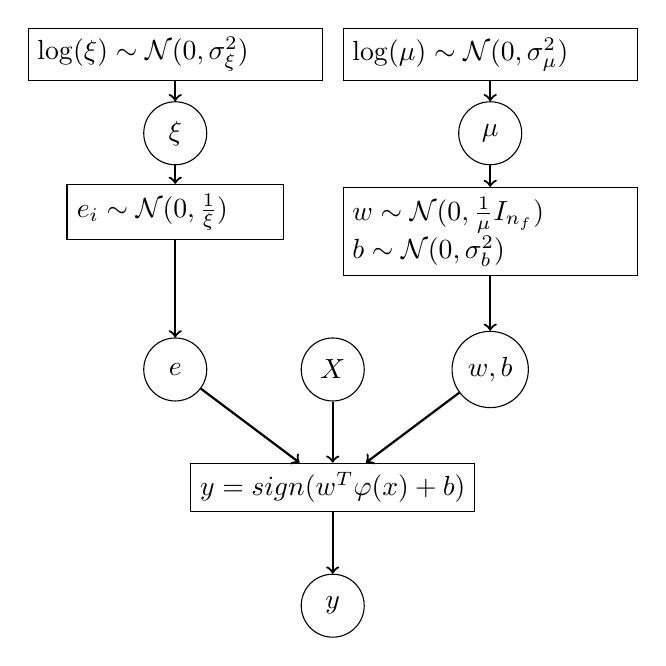
\begin{tikzpicture}
	\tikzstyle{sum} = [draw, circle, minimum size=0.8cm, node distance=1.75cm]
	\tikzstyle{block} = [draw, rectangle, minimum width = 2.75cm, minimum height = 0.5cm]
	\node [sum] (y) at (2,-3) {$y$};
	\node [sum] (eps) at (0,0) {$e$}; 
	\node [sum] (X) at (2,0) {$X$}; 
	\node [sum] (w) at (4,0) {$w,b$};
	\node [block, fill=white] (M) at (2, -1.5) {$y = \text{sign}(w^T \varphi(x) + b)$};
	\node [block, text width=3.5cm] (alpha) at (4,1.75) {$w \sim \mathcal{N}(0,\frac{1}{\mu}I_{n_f})$\\ $b \sim \mathcal{N}(0,\sigma^2_b)$};

	\draw[->,thick] (eps) -- (M);
	\draw[->,thick] (w) -- (M);
	\draw[->,thick] (X) -- (M);
	\draw[->,thick] (M) -- (y);
	%\draw[->,thick] (X) -- (y) node[block, midway, fill=white] {$y = Xw+\varepsilon$};
	\draw[->,thick] (alpha) -- (w);
	\node [block, text width=2.5cm] (lambda) at (0,2) {$e_i \sim \mathcal{N}(0,\frac{1}{\xi})$};
	\draw[->,thick] (lambda) -- (eps);
 
	\node [sum] (mu) at (4,3) {$\mu$};
	\node [sum] (xi) at (0,3) {$\xi$};
	\draw[->, thick] (xi) -- (lambda);
	\draw[->, thick] (mu) -- (alpha);		
	
	\node [block, text width=3.5cm] (vert_mu) at (4,4) {$\log(\mu) \sim \mathcal{N}(0,\sigma_\mu^2)$};		
	\node [block, text width=3.5cm] (vert_xi) at (0,4) {$\log(\xi) \sim \mathcal{N}(0,\sigma_\xi^2)$};	
	
	\draw[->, thick] (vert_mu) -- (mu);
	\draw[->, thick] (vert_xi) -- (xi);	
	
\end{tikzpicture}
\caption{Zusammenfassung der Verteilungs- und Modellannahmen}
\end{figure}
\newpage
Zunächst stellen wir über den Posterior $\mathbb{P}(\log \mu, \log \xi \vert D, K)$ mit Hilfe der Annahmen fest, dass

\begin{align*}
		 \mathbb{P}(\log(\mu), \log(\xi)\vert D, K)
	   &\;=\;\hspace{0.1cm} \frac{\mathbb{P}(D\vert \log(\mu),\log(\xi),K)\mathbb{P}(\log(\mu), \log(\xi) \vert K)}{\mathbb{P}(D\vert K)}  \\
\propto &\; \mathbb{P}(D\vert \log(\mu),\log(\xi),K)\exp(-\frac{x^2}{2\sigma_							  \mu^2})\exp(-\frac{x^2}{2\sigma_\xi^2})\\
\rightarrow & \;\mathbb{P}(D\vert \log(\mu),\log(\xi),K) \text{ für } \sigma_\mu, \sigma_\xi \rightarrow \infty.
\end{align*}

Somit reicht es zum Aufstellen des MAP-Schätzers die Likelihood  $\mathbb{P}(D\vert \log(\mu),\log(\xi),K)$ gegeben der Hyperparameter $\mu, \xi$ zu betrachten. Diese Likelihood, und damit $\mathbb{P}(\log(\mu), \log(\xi)\vert D, K)$, lässt sich weiter mit Hilfe der MAP-Schätzer $(\hat{w}_{MAP}, \hat{b}_{MAP})$ darstellen, was wir in folgendem Lemma zusammenfassen.

\begin{lemma}[Darstellung der a posteriori Wahrscheinlichkeit]

Es gelten die zu Beginn des Kapitels getroffenen Annahmen an $\mu, \xi$. Dann folgt

\begin{align*}
	\mathbb{P}(\log(\mu), \log(\xi)\vert D, K) \propto\; & \mathbb{P}(D\vert \log(\mu),			\log(\xi),K) \\
	\propto\; & \frac{\sqrt{\mu^{n_f} \xi^n}}	{\sqrt{\det H}} \exp(- \mathcal{J}(\hat{w}			_{MAP},\hat{b}_{MAP})),
\end{align*}

wobei 
\begin{center}
	$\mathcal{J}(w,b) = \frac{\mu}{2}w^T w + \frac{\xi}{2}\overset{n}{\underset{i=1}			{\sum}} e_i ^2 \text{ und } H = \begin{pmatrix}
	\frac{\partial^2 \mathcal{J}}{\partial w^2 } & \frac{\partial^2 \mathcal{J}}				{\partial w \partial b } \\
	\frac{\partial^2 \mathcal{J}}{\partial b \partial w } & \frac{\partial^2 					\mathcal{J}}{\partial b^2 }
	\end{pmatrix}.$
\end{center}

\end{lemma}
%VERWEIS AUF VORIGES KAPITEL, GLEICHUNGEN WIE IN DEM LEVELS PAPER

\begin{proof}
Die erste Proportionalität wurde vor Beginn des Lemmas gezeigt, für die zweite siehe \cite{LS-SVM}.
\end{proof}

An dieser Stelle wäre es schon möglich das Optimierungsproblem für die Hyperparameterinferenz zu formulieren, was aufgrund der Determinante $\det H$ zu keinem befriedigenden Ausdruck führt. Dem entgegnen Gestel, Suykens et. al. durch folgende Darstellung der Determinante:

\begin{lemma}[Darstellung der Determinante der Hessematrix]
Betrache die aus dem LS-SVM Problem stammenden Ausdrücke 
\begin{center}
	$\mathcal{J}(w,b) = \frac{\mu}{2}w^T w + \frac{\xi}{2}\overset{n}{\underset{i=1}			{\sum}} e_i ^2 \text{ und } H = \begin{pmatrix}
	\frac{\partial^2 \mathcal{J}}{\partial w^2 } & \frac{\partial^2 \mathcal{J}}				{\partial w \partial b } \\
	\frac{\partial^2 \mathcal{J}}{\partial b \partial w } & \frac{\partial^2 					\mathcal{J}}{\partial b^2 }
	\end{pmatrix}.$
\end{center}

Dann gilt

\begin{center}
	$\det(H) = n \mu^{n_f - N_{eff}} \xi \underset{i=1}{\overset{N_{eff}}{\prod}}(\mu + 			\xi \lambda_i)$,
\end{center}

wobei $N_{eff}$ die Anzahl der Eigenwerte $\lambda_i$ ungleich Null der zentrierten Matrix $M \Omega M$ mit
\begin{center}
	$\Omega_{i,j} = K(x_i, x_j)$ und $M = I_n + \frac{1}{n} 1_v 1_v^T$ ist.
\end{center}
\end{lemma}

\begin{proof}
Siehe \cite{LS-SVM}, Appendix B.
\end{proof}

Beide darstellenden Lemmata lassen sich nun bei einem MAP-Schätzer Ansatz kombinieren und ergeben eines der Hauptresultate zur LS-SVM:


\begin{theorem}[Hyperparameterinferenz der LS-SVM]

Seien die Voraussetzungen an a priori Verteilungen wie zu Beginn des Kapitels.\\
(i) Dann sind die MAP-Schätzer der Hyperparameter $\mu, \xi$ gegeben durch

\begin{align*}
	(\hat{\mu}_{MAP}, \hat{\xi}_{MAP}) &\;=\; \underset{\mu, \xi}{\arg \min}  \hspace{0.2cm}		\mathcal{J}(\hat{w}_{MAP}, \hat{b}_{MAP}) + \frac{1}{2}\sum_{i=1}^{N_{eff}}\log(\mu 		+ \xi \lambda_i) \\
	 & \hspace{0.8cm}- \frac{N_{eff}}{2}\log(\mu) - \frac{n -1 }{2}\log(\xi)\\
	&\;=:\; \underset{\mu, \xi}{\arg \min} \hspace{0.2cm}	\mathcal{J}_\text{hyp}(\mu, \xi)
\end{align*}



mit dem Ausgangsfunktional der LS-SVM 
$\mathcal{J}(w,b) = \frac{\mu}{2}w^T w + \frac{\xi}{2}\overset{n}{\underset{i=1}{\sum}} e_i ^2$,
sowie den nichttrivialen Eigenwerten $\lambda_i$ der zentrierten Kernelmatrix.

(ii) Weiterhin sind die partiellen Ableitungen des Zielfunktionals gegeben durch

\begin{align*}
	\frac{\partial \mathcal{J}_\text{hyp}}{\partial \mu} &\;=\; \hat{w}_{MAP}^T \hat{w}			_{MAP} + \frac{1}{2} \overset{N_{eff}}{\underset{i=1}{\sum}} \frac{1}{\mu + \xi 			\lambda_i} - \frac{N_{eff}}{2\mu} \\
    \frac{\partial \mathcal{J}_\text{hyp}}{\partial \xi} &\;=\; \overset{n}						{\underset{i=1}{\sum}}( y_i - (\hat{w}_{MAP}^T \varphi(x_i) + \hat{b}_{MAP}))^2 + \overset{N_{eff}}{\underset{i=1}{\sum}} \frac{\lambda_i}{\mu + \xi \lambda_i} - \frac{N-1}{2\xi}.
\end{align*} 
\end{theorem}

\begin{proof}
Wir verwenden die beiden vorausgegangenen Lemmata und erhalten durch einsetzen und der Definition des MAP-Schätzers, sowie negativer log-Transformation:
\begin{align*}
	(\hat{\mu}_{MAP}, \hat{\xi}_{MAP}) 
	&\;=\; \underset{\mu, \xi}{\arg \max}\; \mathbb{P}(\mu, \xi \vert D, K) \\
	&\;=\; \underset{\mu, \xi}{\arg \max}\; \mathbb{P}(\log(\mu) \log(\xi) \vert D, K) \\
	& \hspace{-0.5cm}\;\overset{\text{Lemma 15}}{=}\; \underset{\mu, \xi}{\arg \max}\; \mathbb{P}(D \vert \log(\mu), \log(\xi), K) \\
	&\hspace{-0.5cm}\;\overset{\text{Lemma 15}}{=}\; \underset{\mu, \xi}{\arg \max}\; \frac{\sqrt{\mu^{n_f} \xi^n}}	{\sqrt{\det H}} 				\exp(- \mathcal{J}(\hat{w}_{MAP},\hat{b}_{MAP})) \\
	&\hspace{-0.5cm}\;\overset{\text{Lemma 16}}{=}\; \underset{\mu, \xi}{\arg \max}\; \frac{\sqrt{\mu^{n_f} \xi^n}}	{\sqrt{n \mu^{n_f - 			N_{eff}} \xi \underset{i=1}{\overset{N_{eff}}{\prod}}(\mu + 			\xi 				\lambda_i)}} \exp(- \mathcal{J}(\hat{w}_{MAP},\hat{b}_{MAP})) \\
	&\;=\; \underset{\mu, \xi}{\arg \max}\; \frac{\sqrt{\mu^{N_{eff}} \xi^{n-1}}}	{\sqrt{ 				\underset{i=1}{\overset{N_{eff}}{\prod}}(\mu + 	\xi	\lambda_i)}} \exp(- 					\mathcal{J}(\hat{w}_{MAP},\hat{b}_{MAP})) \\
	&\;=\; \underset{\mu, \xi}{\arg \min}\;  \hspace{0.2cm} \mathcal{J}(\hat{w}_{MAP}, 			   	 	\hat{b}_{MAP}) + \frac{1}{2}\sum_{i=1}^{N_{eff}}\log(\mu + \xi \lambda_i)\\
	 & \hspace{0.8cm}- \frac{N_{eff}}{2}\log(\mu) - \frac{n -1 }{2}\log(\xi),
\end{align*}

was uns (i) liefert. (ii) erhalten wir direkt durch partielles Ableiten.

\end{proof}

Dieses Minimierungsproblem ermöglicht es die Wahl der Hyperparameter mit Hilfe eines rigorosen Verfahrens zu treffen, statt durch Tuning per Hand und verschiedenen anderen heuristischen Methoden. Um das Zielfunktional aufzustellen benötigt man die Eigenwerte $\lambda_i$ der zentrierten Kernelmatrix. Es fällt auf, dass die Größe der zentrierten Kernelmatrix mit der Größe des Datenvektors $D$ wächst, so dass bei großen Datenmengen extrem viele Eigenwerte auftreten können. In der Praxis wird dem begegnet, indem man approximativ die größten Eigenwerte berechnet und so das Zielfunktional annähert. Dies geschieht beispielsweise, sogar bei unendlichdimensionalem Feature-Space, mit einem Expectation-Maximization-Algorithmus, siehe etwa \cite{Kernel_PCA}. Für umfassende Details zur Spektraltheorie von Kernen im Rahmen des Machine Learning verweisen wir auf \cite{spectral_kernel}.

%Algorithmen zur Lösung???

%SKALARES PROBLEM?

\subsection{Kernelselektion}

Nachdem wir eine mögliche Antwort auf die Frage der Auswahl von Hyperparametern gegeben haben, wollen wir uns mit der auf der nächst höheren Ebene liegenden Frage der Kernelselektion beschäftigen. Im Allgemeinen ist die Wahl des Kernels zum durchführen des Kerneltricks im Rahmen der nichtlinearen Trennung mittels LS-SVM höchst nicht-trivial. Wir verwenden, nach \cite{LS-SVM}, den Ansatz die Kernel $K_i$ und die jeweils zugehörige LS-SVM mit ihren Parametern $w_i, b_i, \mu_i, \xi_i$ als verschiedene Modelle zu betrachten, und Modellauswahl traditionell bayesianischer Art durchzuführen. Für eine umfassende Einführung in Techniken der Bayesianischen Modellselektion empfehlen wir \cite{Bayes_model_selection}. Im folgenden Stellen wir den recht simplen Ansatz von Gestel, Suykens et. al. vor.

Ein Ansatz der Bayesianische Modelselektion basiert auf einem Ranking der Kernel durch die zugehörige a posteriori Modellevidenz $\mathbb{P}(K_i\vert D)$. Wir beschränken uns hier auf die Auswahl unter endlich vielen Kernen $\{K_i\}_{i=1,...,m}$. Die Auswahl wird durch die Wahl des Kernels mit der größten Evidenz $\mathbb{P}(K_i\vert D)$ getätigt. Da wir nur endlich viele Kernel zur Auswahl stellen, läuft dies auf ein heuristisches auswählen und sortieren hinaus.

Ähnlich wie in den vorangegangenen Betrachtungen platzieren wir a priori Verteilungen, diesmal auf die Kernel $K_I$ selber. Dabei nehmen wir an:

\begin{itemize}
	\item Platziere (diskrete) a priori Verteilung auf die Kerne $K_i$:
		\begin{align*}
		\mathbb{P}(K_i) = p_i,\quad \sum_{i=1}^{m} \mathbb{P}(K_i) = 1
		\end{align*}
	\item Nehme eine Gleichverteilung an, d.h. $p_i = p_j$ für alle $i,j = 1,\dots,M$.
	\item Seien die Hyperparameter $\mu_i, \xi_i$ der jeweiligen Models mit Kern $K_i$ 				  stochastisch unabhängig und haben folgende Verteilung:
		  \begin{align*}
				\log(\mu_i) \sim \mathcal{N}(0, \sigma_{\mu_i}^2), \quad\log(\xi_i) \sim 						\mathcal{N}(0, \sigma_{\xi_i}^2)
		  \end{align*}
	\item $\sigma_{\mu_i}^2, \sigma_{\xi_i}^2 \rightarrow \infty$ für alle $i = 1,\dots,M				   $.
\end{itemize}

Es ist auch möglich ganze Familien von Kerneln zu betrachten, und unter diesen zu Selektieren. Ein Beispiel wäre die Wahl des geeigneten Kernelparameters eines RBF-Kerns. Diese Fragestellung führt jedoch zu nicht-trivialen Minimierungsproblem in dem Sinne, dass keine einfache Heuristik zur Wahl des optimalen Kernels verwendet werden kann.

Der folgende Satz gibt als weiteres Hauptresultat an, wie man die Evidenzen $\mathbb{P}(K_i \vert D)$ in Proportionalität berechnen kann, und somit Kernel selektieren kann.


\begin{theorem}[Berechnung der Evidenz zur Kernelselektion]
Seien die obigen Annahmen erfüllt. Weiterhin sei ein Datenvektor $D$ gegeben, so dass die a posteriori Verteilungen $\mathbb{P}(\log(\mu),\log(\xi) \vert D, K_i)$ eine positiv definite Kovarianzmatrix besitzt. Dann gilt:

\begin{align*}
	\mathbb{P}(K_i \vert D) 
	&\propto \mathbb{P}(D \vert K_i)\\
 	&\propto \mathbb{P}(D \vert \log(\hat{\mu}_{i_{MAP}}), \log(\hat{\xi}_{i_{MAP}}), 			K_i)\frac{\sigma_{\mu_i\vert D} \sigma_{\xi_i\vert D}}{\sigma_{\mu_i} 						\sigma_{\xi_i}}\\
	&\propto \sqrt{\frac{\hat{\mu}^{N_{eff}}_{i_{MAP}} \hat{\xi}^{n-1}_{i_{MAP}}}				{(\gamma_{eff}-1)(n - \gamma_{eff}) \prod_{j=1}^{N_{eff}}(\hat{\mu}_{i_{MAP}} + 			\hat{\xi}_{i_{MAP}}\lambda_j)}}
\end{align*}

wobei $\gamma_{eff} = 1 + \sum_{j=1}^{N_{eff}}\frac{\hat{\xi}_{i_{MAP}}\lambda_j}{\hat{\mu}_{i_{MAP}} + \hat{\xi}_{i_{MAP}}\lambda_j}$.

\end{theorem}

\begin{proof}
Die erste Proportionalität ergibt sich durch die Gleichverteilungsannahme an die $K_i$ und Definition des Posteriors

\begin{center}
	$\mathbb{P}(K_i \vert D) = \frac{\mathbb{P}(D\vert K_i)\mathbb{P}(K_i)}{\mathbb{P}			(D)}
	\propto \mathbb{P}(D \vert K_i)$.
\end{center}
Für den Rest verweisen wir auf \cite{LS-SVM}.
\end{proof}

Der Faktor $\frac{\sigma_{\mu_i\vert D} \sigma_{\xi_i\vert D}}{\sigma_{\mu_i} 						\sigma_{\xi_i}}$ wird auch mit Occam's Faktor bezeichnet, benannt nach dem mittelalterlichen Philosophen Wilhelm von Ockham, auf den auch der bekannte Begriff der Occam'schen Rasierklinge zurückgeht. Bemerkenswert an der obigen proportionalen Darstellung ist, dass sobald man MAP-Schätzer und Eigenwerte aus vorangehender Analyse gebildet hat, die Modellevidenz im Proportionalen sofort berechnet werden kann. Bei Optimierung hinsichtlich ganzer Kernelfamilien ließe sich diese Proportionalität als Ansatz nutzen um ein Minimierungsproblem herzuleiten.

Zusammenfassend münden die vorgestellten Theoreme in folgendem Algorithmus zur Selektion von Kernen bei der LS-SVM:

\begin{center}
	\begin{figure}
		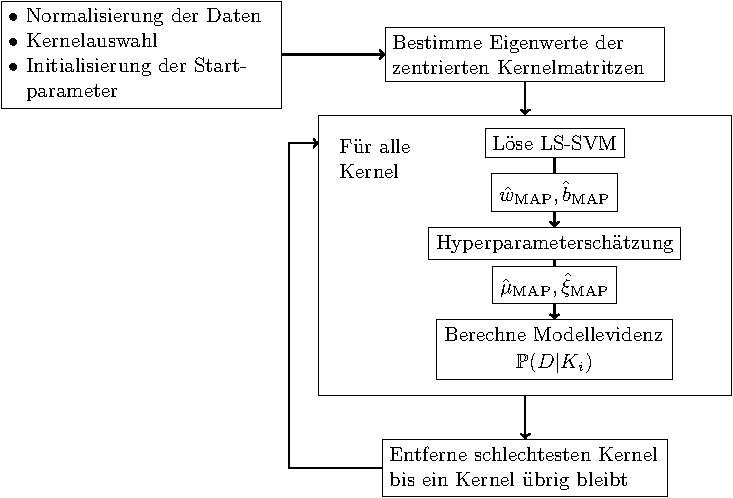
\includegraphics[scale=0.9]{Algo.pdf}
		\caption{Algorithmus zur Kernelselektion bei der LS-SVM}
	\end{figure}
\end{center}

\newpage
\thispagestyle{plain}
\noindent\textbf{Fazit \& Ausblick}\\
Wie wir exemplarisch gezeigt haben, lässt sich die Bayes-Theorie gewinnbringend im Kontext des Machine Learnings verwenden. Der Hauptnutzen besteht darin, numerisch umsetzbare Problemklassen rigoros herleiten zu können. Weiterhin lassen sich Probleme, wie das Hyperparametertuning und die Modellselektion, durch fundierte Ansätze statt bloßer Heuristik angehen. An diesem Punkt stellt sich uns die Frage, aus welchem Grund diese Art von Ansätzen selten in der Praxis Verwendung zu finden scheinen. Gründe hierfür könnten zum einen sein, dass für jedes individuelle Problem eine eigenständige Bayesianische Analyse nötig ist, was zeit- und arbeitsaufwändig ist. Zum anderen könnte es daran liegen, dass die Mischung aus Statistik und Numerik als Schnittstellenbereich zu wenig Aufmerksamkeit bekommt, und deshalb nicht verbreitet ist. Und schlussendlich kann es natürlich auch sein, dass uns nicht bekannte Nachteile bei den verwendeten Ansätzen bestehen. Im Blick auf die Zukunft des Machine Learnings wäre eine Grundlagentheorie und eine detaillierte, mathematisch saubere Untersuchung der zugrunde liegenden Prinzipien wichtig. Die Bayes-Theorie kann hierzu das mathematische Bindeglied zwischen der Statistik, der Numerik und Data Science sein. Da die Probleme und Prinzipien des Machine Learning von Natur aus ein holistisches Denken verlangen, wird eine Zusammenarbeit dieser Sparten immer wichtiger.